\documentclass[10pt,a4paper,final]{article}
\usepackage[utf8]{inputenc}
\usepackage[french]{babel}
\usepackage[T1]{fontenc}
\usepackage{amsmath}
\usepackage{amsfonts}
\usepackage{amssymb}
\usepackage{listings}
\usepackage{fancyhdr}
\usepackage{graphicx}
\usepackage{xcolor}
\author{Léo Boisson}
\setlength\parindent{24pt}
\title{\textbf{Compte rendu TP2/3 Réseau}}
\makeindex
\pagestyle{fancy}
\lhead{BOISSON Léo}
\rhead{Compte-rendu TP Réseau}
\cfoot{\thepage}
\renewcommand{\headrulewidth}{0.4pt}
\renewcommand{\footrulewidth}{0.4pt}

\lstset{language=C,
                basicstyle=\footnotesize,
                keywordstyle=\color{blue}\ttfamily,
                stringstyle=\color{red}\ttfamily,
                keywordstyle=\bfseries\color{green!40!black},
                commentstyle=\itshape\color{purple!40!black},
                identifierstyle=\color{blue},
                breaklines=true,
				frame=trbl,
				numbers=left,
 				xleftmargin=\parindent,
                morecomment=[l][\color{magenta}]{\#}
}

\begin{document}
\date{}
\maketitle  
\tableofcontents  
\newpage



\section{Introduction} 

	\subsection{Historique}
		Les sockets sont un ensemble de fonctions de communications, proposés en 1980 pour le \textbf{Berkeley Software Distribution} (BSD), en open source, par 								l'université de Berkeley. Elles permettent a des applications de se connecter entre elles, via un principe client/serveur.	\\
		Aujourd'hui, les sockets sont disponibles dans quasiment tous les langages de programmations, et font offices de norme.\\
		On distingue deux modes de communication avec les sockets :\\
		\begin{itemize}
			\item
				Le mode connecté, qui utilise le protocole TCP. Dans ce mode, une connexion durable est établie entre les deux processus, afin que l'adresse de destination ne 							soit pas nécessaire à chaque envoie de données.
			\item
				Le mode non-connecté, qui utilise le protocole UDP. Ce mode nécessite l'adresse de destination à chaque envoi, et il n'y a pas de confirmation du bon envoi des
				données. Ce mode est plus adapté à l'envoi de flux audio ou vidéo.
		\end{itemize}+
		
	\subsection{Objectif du TP}
		L'objectif de ce TP est d'aborder le développement de sockets, et de se familiariser avec les outils qui vont avec (les primitives). Pour cela, nous allons 
		programmer des applications client/serveur basique, pour ensuite observer et analyser les échanges de données entre ces applications.
	
	
\section{Application client/serveur echo}
	\subsection{principe de fonctionnement}
		Nous réalisons une application de type client/serveur, afin de calculer le temps que mets une requête du client à parvenir au serveur, à être traitée, puis à revenir au 				client. Nous utilisons la primitive \textit{\textrm{gettimeofday}}, qui renvoie l'heure en secondes et microsecondes (avec la zone temporelle passée en argument).\\
		En utilisant cette fonction deux fois dans le code du client, une première fois lors de l'envoi au serveur, et une seconde lors de la réception depuis le serveur, il nous 				suffit de soustraire la première à la seconde pour obtenir le temps d'aller et retour d'une requête.
				
	\subsection{Code source du client}
		On constateras les \textit{\textrm{gettimeofday}}, lignes 81 et 104.
		\lstinputlisting{client_echo.c}
		
	\subsection{Code source du serveur}
		Le serveur ne fait que réceptionner le message du client, un "echo", et le renvoi immédiatement.
		\lstinputlisting{server_echo.c}

	\subsection{Analyse des trames réseau}
		Les programmes affichent ceci dans le terminal :\\
		
		\begin{figure}[!h] 
			\centering
			\caption{Pour le serveur :}
			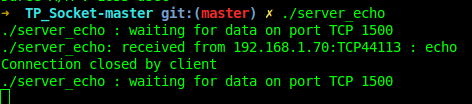
\includegraphics[scale=0.5]{img/server_echo_terminal.png} 
			\caption{Pour le client :}
			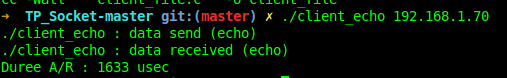
\includegraphics[scale=0.5]{img/client_echo_terminal.png} 
		\end{figure}
		\newpage
		
		Ensuite, nous regardons les trames échangées avec wireshark, en utilisant un filtre sur le port. Nous obtenons ceci :\\
		\begin{figure}[!h] 
			\centering
			\caption{Affichage dans wireshark :}
			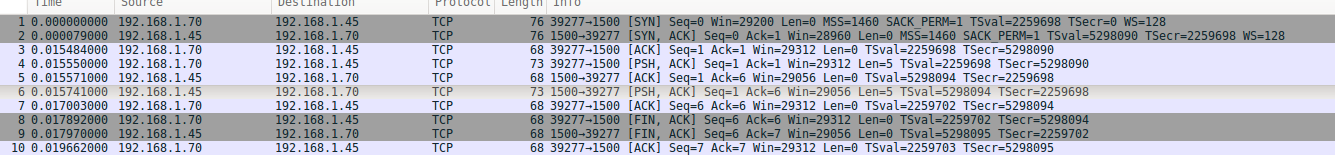
\includegraphics[scale=0.3]{img/wireshark_echo.png} 
		\end{figure}		
		\newline
		Que nous pouvons analyser plus facilement en utilisant l'option \textit{\textrm{flowchart}} dans wireshark :\\
		\begin{figure}[!h] 
			\centering
			\caption{Flowchart de echo :}
			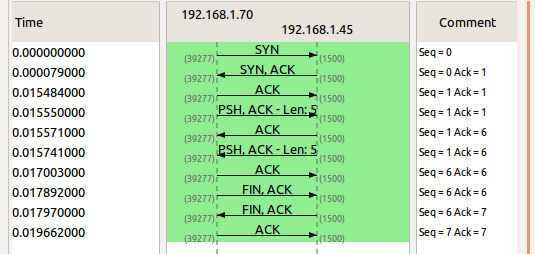
\includegraphics[scale=0.5]{img/flowchart_echo.png} 
		\end{figure}	
		\newline
		Les trois premiers paquets correspondent au mécanisme de \textit{\textrm{handshake}}. Ensuite, on voit un paquet de taille 5 aller du client au serveur. Il s'agit
		du "echo" (4 caractères + le retour chariot).\\
		\newline
		Ensuite, le serveur envoi l'accusé de réception, avec le numéro d'acquittement 6 (5+1), puis il envoi la sa réponse à la requête, soit le message "echo".
		le numéro d'acquittement n'as pas changé, puisque le serveur n'as pas reçu d'autre données entre temps. \\
		S’en suit alors le paquet 7 envoyé par le client qui accuse réception du retour effectué par le serveur. Le numéro d’acquittement est devenu 6 (1+6) pour le 
		client (il a reçu 5 caractères).\\
		\newline
		Le client engage alors le processus de terminaison de la connexion. Il envoie un paquet vide avec le drapeau FIN. Le serveur lui renvoie 
		alors un paquet similaire en incrémentant le numéro d’acquittement de 1. Enfin, un dernier paquet est transmis au serveur par le client en tant qu'accusé de 
		réception du retour du paquet FIN. La connexion est alors terminée.\\
		\newpage		
		
\section{Application client/serveur chifoumi}


\section{Échange de données entre deux machines}


\section{Analyse par Wireshark}


\section{conclusion}


\end{document}s